\documentclass[11pt]{article}
\usepackage[T1]{fontenc}
\usepackage{lmodern}
\usepackage{amsmath,amsthm,amssymb,mathtools}
\usepackage[margin=1.05in]{geometry}
\usepackage{microtype}
\usepackage{xcolor,enumitem,booktabs}
\usepackage{tikz}
\usetikzlibrary{arrows.meta,positioning}
\definecolor{linkblue}{rgb}{0.05,0.16,0.42}
\usepackage[colorlinks=true,linkcolor=linkblue,citecolor=linkblue,urlcolor=linkblue]{hyperref}
\usepackage[capitalise,noabbrev]{cleveref}
\hypersetup{pdftitle={Deterministic quasipolynomial-time mean-payoff games},pdfauthor={OpenAI}}
\pdftrailerid{}
\setlength{\emergencystretch}{1.5em}
\setlist[enumerate]{itemsep=.45em,topsep=.5em}
\setlist[itemize]{itemsep=.25em,topsep=.4em}
\numberwithin{equation}{section}
\theoremstyle{plain}
\newtheorem{theorem}{Theorem}[section]
\newtheorem{lemma}[theorem]{Lemma}
\newtheorem{proposition}[theorem]{Proposition}
\newtheorem{corollary}[theorem]{Corollary}
\theoremstyle{definition}
\newtheorem{definition}[theorem]{Definition}
\newtheorem{procedure}[theorem]{Procedure}
\theoremstyle{remark}
\newtheorem{remark}[theorem]{Remark}
\newcommand{\Z}{\mathbb Z}
\newcommand{\Q}{\mathbb Q}
\DeclareMathOperator{\clip}{clip}
\DeclareMathOperator{\MP}{MP}
\newcommand{\Label}{\ensuremath{\mathsf{Label}}}
\newcommand{\Basic}{\ensuremath{\mathsf{Basic}}}
\newcommand{\hi}{\mathrm{hi}}
\newcommand{\lo}{\mathrm{lo}}

\title{Deterministic quasipolynomial-time mean-payoff games}
\author{OpenAI}
\date{September 25, 2026}
\begin{document}
\maketitle
\begin{abstract}
We give a deterministic algorithm that computes the complete zero-threshold
winning set of a finite mean-payoff game with arbitrary signed integer edge
weights encoded in binary. For total explicit input length $L$, it uses
$2^{O((\log(L+2))^2)}$ bit operations. A reduction also computes the exact
rational value at every vertex and globally optimal positional strategies
for both players within the same quasipolynomial bound.
\end{abstract}
\setcounter{tocdepth}{1}
\hypersetup{bookmarksdepth=2}
\tableofcontents
\clearpage
\section{Introduction}
\label{sec:introduction}

In a mean-payoff game, two players choose edges of a finite graph and
compete over the long-run average weight of the resulting infinite
walk. The objective is numerical, but the question of who can enforce
a nonnegative average is a finite decision problem. A central
algorithmic issue is the representation of the weights: a procedure
polynomial in their absolute values may take exponential time in the
length of the input. We give a deterministic algorithm whose running
time is quasipolynomial in that binary length and which determines
all winning starting vertices together.

\subsection{The problem and the main theorem}

Let $G=(V,E)$ be a finite directed graph with
$V=\{1,\ldots,n\}$ and $n\ge1$. Each vertex has at least one
outgoing edge and belongs to exactly one of
$V_{\mathrm{Max}}$ and $V_{\mathrm{Min}}$. The edge weights
$w:E\to\Z$ are arbitrary signed binary integers. Self-loops and
parallel edges are allowed; parallel edges are separate entries of
the explicit edge list. At a vertex its owner chooses the next edge.
Both players' strategies may depend on the entire finite history.
For an infinite play $\pi=(e_0,e_1,\ldots)$, write
\[
 \MP_w(\pi)=\liminf_{T\to\infty}\frac1T
                         \sum_{t=0}^{T-1}w(e_t).
\]
We count the complete input length $L$ in a fixed conventional binary
encoding of the graph, endpoints, ownership, and weights. For a start
$v$ and strategies $\sigma,\tau$, denote their induced play by
$\pi_{v,\sigma,\tau}$.

\begin{theorem}\label{thm:main}
A uniform deterministic algorithm returns exactly the set
\[
 U=\bigl\{v\in V:\exists\text{ Max strategy }\sigma\ 
       \forall\text{ Min strategies }\tau,
       \ \MP_w(\pi_{v,\sigma,\tau})\ge0\bigr\}
\]
for every game specified above. For an absolute constant $C>0$, the
complete computation uses at most
\[
                      2^{C(\log_2(L+2))^2}
\]
bit operations in a standard model polynomially equivalent to a
uniform deterministic Turing machine. The bound includes
preprocessing, exact arithmetic, recursion, and output of the entire
set $U$.
\end{theorem}

A positional strategy chooses its outgoing edge using only the current
vertex. Section~\ref{sec:full-solution} derives the exact rational
value at every starting vertex and globally optimal positional
strategies for both players, within the same quasipolynomial bit bound.
Section~\ref{sec:energy-credits} decides whether a prescribed initial
credit can keep every finite accumulated weight nonnegative in a
one-resource energy game, and computes minimum winning credits. Section~\ref{sec:tropical}
applies classical reductions to tropical feasibility and fixed-corank
tropical-rank tests. A polynomial bound for the complete binary input
would be a further improvement.

\subsection{Earlier algorithms and binary weights}

Ehrenfeucht and Mycielski proved the existence of positional optimal
strategies for mean-payoff games~\cite{EhrenfeuchtMycielski1979}.
Positional determinacy places the threshold problem in
$\mathrm{NP}\cap\mathrm{coNP}$. Zwick and Paterson developed
pseudopolynomial algorithms and complexity reductions
\cite{ZwickPaterson1996}. Such bounds
can be polynomial in the number of vertices and the largest absolute
weight while remaining exponential in the binary encoding length.
This distinction is central to Theorem~\ref{thm:main}.

The energy formulation asks whether a finite initial credit can keep
all finite accumulated weights nonnegative. Brim, Chaloupka, Doyen,
Gentilini, and Raskin developed bounded integer progress measures and
monotone lifting, with an $O(|E|nW_0)$ threshold and winning-region
bound when $W_0$ bounds the absolute weights
\cite[Theorem~8]{BrimEtAl2011}.
Dorfman, Kaplan, and Zwick developed a deterministic exponential-time
approach based on accelerated potential updates and scaling; Austin
and Dell'Erba corrected its update procedure
\cite{DorfmanKaplanZwick2019,AustinDellErba2023}. Kozachinskiy
gives a polyhedral interpretation and a weight-independent
$n^{O(1)}2^{n/2}$ arithmetic bound for energy winners
\cite{Kozachinskiy2021}.

Strategy-improvement algorithms provide another important comparison.
Bj\"orklund and Vorobyov proved an expected
$2^{O(\sqrt{n\log n})}$ arithmetic bound for the threshold partition
on graphs without parallel edges
\cite[Theorem~7.1]{BjorklundVorobyov2007}, following work with
Sandberg~\cite{BjorklundSandbergVorobyov2004}.
Recent analyses concern Random-Action-Removal~\cite{Zwick2026} and
Switch-All and Random-Edge for energy games
\cite{DorfmanKaplanZwick2026}. Iteration counts and arithmetic bounds
must be distinguished from bit bounds: strategy evaluation and the
sizes of intermediate numbers contribute to the latter.

Parity games use an extremal priority occurring infinitely often to
determine the winner. They reduce in polynomial time to mean-payoff
threshold games using weights of exponential magnitude but polynomial
binary length~\cite[Section~3]{Jurdzinski1998}. Calude, Jain,
Khoussainov, Li, and Stephan gave
a quasipolynomial algorithm for parity games
\cite{CaludeJainKhoussainovLiStephan2022}. The reduction goes from
parity to mean payoff, so this result does not by itself give a
quasipolynomial algorithm for arbitrary binary-weight mean-payoff games.
Daviaud, Jurdzi\'nski, and Lazi\'c combined succinct parity progress
measures with energy bounds in a pseudo-quasipolynomial algorithm for
mean-payoff parity games~\cite{DaviaudJurdzinskiLazic2018}; that
bound still contains a numerical weight parameter. Smoothed polynomial
results for independent Gaussian perturbations of payoffs on ergodic
game graphs concern a different input model~\cite{LoffSkomra2024}.

\subsection{How the proof works}

An integer potential assigns a number to each vertex. First replace
$w(e)$ by $\widehat w(e)=(n+1)w(e)+1$, which makes every simple
cycle sum nonzero while separating negative original sums from
nonnegative ones. For $z\in\Z^V$, let $F_i(z)$ be the maximum
of $\widehat w(e)+z_j$ over edges $e:i\to j$ at a Max vertex,
and the minimum at a Min vertex. For integer vectors $A\le u$,
the box $[A,u]$ consists of all integer vectors between them,
coordinatewise. In this box,
a subsolution is a vector $x\in[A,u]$ satisfying $x_i\le F_i(x)$
wherever $x_i>A_i$; a supersolution is a vector $y\in[A,u]$
satisfying $y_i\ge F_i(y)$ wherever $y_i<u_i$.
Clipping a vector to the box means replacing coordinate $z_i$ by
$\min\{u_i,\max\{A_i,z_i\}\}$. The comparison theorem in
\emph{Randomized quasipolynomial-time mean-payoff games}, our
companion article, gives a unique fixed point $h$ of $z\mapsto\min\{u,\max\{A,F(z)\}\}$,
and the inequalities $x\le h\le y$ for every such pair. These
finite-box facts and their basic iteration procedure are the only
results imported from the companion in the proof of
Theorem~\ref{thm:main}
\cite[Definition~2.2 and Lemmas~2.3--2.4]{OpenAI2026Randomized}.
Section~\ref{sec:boxes} states that interface in full.

The same section places each coordinate of $h$ near one of the
two boundaries of a sufficiently wide box $[0,D]^V$. The upper band
is winning for Max and the lower band for Min. Iterating the clipped
operator from the bottom can require a number of steps proportional
to the numerical width $D$. We instead ask which boundary labels are
forced, without computing $h$.

For a box $[A,A+D]$, give the vertices positive rational masses
$a_i$ and $b_i$. For a vertex set $S$, its masses are
$a(S)=\sum_{i\in S}a_i$ and $b(S)=\sum_{i\in S}b_i$. A Max witness is a subsolution whose support
$\{i:x_i>A_i\}$ has $a$-mass at most one; it requires a positive
label at coordinates near the upper boundary. A Min witness is the
dual supersolution with support $\{i:y_i<A_i+D\}$ of $b$-mass
at most one; it requires a negative label near the lower boundary.
The task is to meet every requirement of every witness at once. With
initial masses $1/n$, the box solution qualifies on both sides, so
these requirements determine every vertex's winner.

To solve that task recursively, we move an integer pivot vector $k$
near the middle of the box. For a Max witness, a common translation
aligns the largest deviation $x_i-k_i$ with the top of a narrower
box centered at $k$. Clipping at the bottom leaves only coordinates
whose deviations are close to that largest value. A dual operation
handles Min witnesses. Section~\ref{sec:translations} proves that
these operations preserve the required inequalities and restrict
supports to subsets of the original supports.

The algorithm in Section~\ref{sec:algorithm} first moves $k$
downward, then upward. Narrow recursive calls choose which
coordinates move. Each pass protects the extremal deviation of all
witnesses of one type. When a pass stops, any still-needed witness
of the other type must have a set of coordinates close to an extremum
with $a$-mass greater than $3/4$ for a Max witness or $b$-mass
greater than $3/4$ for a Min witness. Otherwise the last recursive call would have
forced another movement. This use of the final, stationary call is
the key deterministic certificate.

One call on a half-width box labels those large-mass sets. Its labels
need not settle the original boundary requirements. They instead
specify new masses: coordinates labelled in a witness's favor become
lighter, and the others heavier. Section~\ref{sec:correctness}
shows that every unsettled witness still has support mass at most
one. Meanwhile, every product $a_i b_i$ increases by a fixed factor.
Once every product exceeds one, each coordinate is excluded from
at least one type of witness support, and the labels can be chosen
directly. Starting with masses $1/n$, only $O(\log(n+1))$ such
product increases can therefore occur along a branch. The final call
on the original box uses the reweighted masses to settle the remaining
requirements. Every child except the half-width call increases the
products; that exceptional child instead reduces the width.
Section~\ref{sec:complexity} counts the possible positions of the
product increases along a branch and bounds the exact arithmetic in
each call, giving the stated bit complexity.

\subsection{Potential methods and recursive precision}

Gurvich, Karzanov, and Khachiyan developed potential transformations
in their algorithm for cyclic games
\cite{GurvichKarzanovKhachiyan1988,KarzanovLebedev1993}: adding
differences of endpoint potentials to edge weights preserves cycle
sums while changing the local inequalities. Paired potentials appear
in the work of Lifshits and Pavlov~\cite{LifshitsPavlov2007}.
Cadilhac, Casares, and Ohlmann give a general framework for accelerated
value iteration~\cite{CadilhacCasaresOhlmann2025}. These methods and
the progress-measure approach described above provide the setting
for our finite-box inequalities.

The closest recursive ancestry is Parys's reduced-precision parity
algorithm~\cite[Algorithm~2, Section~5, and Lemma~6.1]{Parys2019}
and its development by Lehtinen, Parys, Schewe, and Wojtczak
\cite{LehtinenParysScheweWojtczak2022}. Their guarantees protect
all dominions---sets within which one player can keep play and win---
within specified size bounds, and their recursion
separates one child retaining full precision from children of reduced
precision. We likewise use simultaneous obligations for small objects,
but smallness here means rational mass of a potential's support.
Translation near an extremal deviation, the stationary-pivot
certificates, and reweighting establish the needed progress for that
notion of smallness.

Ohlmann's symmetric mean-payoff recursion supplies closely related
potential-based context~\cite{Ohlmann2026}; its subexponential time
analysis is left open in the cited version. Jurdzi\'nski, Morvan,
Ohlmann, and Thejaswini use two simultaneous labellings for symmetric
acceleration of parity algorithms
\cite{JurdzinskiMorvanOhlmannThejaswini2020}; a related development
by Thejaswini, Ohlmann, and Jurdzi\'nski retains both decompositions
to accelerate symmetric recursion~\cite{ThejaswiniOhlmannJurdzinski2022}.
Arnold, Niwi\'nski, and Parys study recursive interval restriction in a
quasipolynomial black-box algorithm for nested fixed-point evaluation
\cite{ArnoldNiwinskiParys2021}. Their bound is expressed in
Boolean-lattice dimension and fixed-point nesting depth. The integer
box here has chains of length $nD+1$, so that result does not directly
give the dependence on $\log D$ established by our translation and
mass arguments.

Fijalkow, Gawrychowski, and Ohlmann studied mean-payoff value iteration
using universal graphs and lower bounds for those representations
\cite{FijalkowGawrychowskiOhlmann2020}. Those lower bounds constrain
universal-graph representations. The present recursion constructs and
reweights boxes for the given instance without using such a representation.

The companion algorithm~\cite{OpenAI2026Randomized} returns potential
vectors with probabilistic comparison guarantees stated separately
for each fixed admissible vector. Here the recursive guarantee is
simultaneous over all qualifying witnesses and concerns their boundary
labels. The two algorithms share the finite-box theory stated in
Section~\ref{sec:boxes}; the companion's randomized proof is
independent of the deterministic recursion. Section~\ref{sec:full-solution}
also explains how its winning-set interface yields randomized exact
values and positional strategies.

\section{From potential comparisons to a labelling problem}
\label{sec:boxes}

This section specifies the finite-box input used from the companion,
then proves the game reduction at the width required by our recursion.
The outcome is a labelling problem whose obligations are expressed by
potential vectors. Later sections solve that problem without finding
the potential that certifies the winning partition.

\subsection{The common finite-box interface}

Fix the input graph and ownership throughout. Following the integer
cycle perturbation of Bj\"orklund and Vorobyov
\cite[Section~9]{BjorklundVorobyov2007}, put
\begin{equation}
 \widehat w(e)=(n+1)w(e)+1,
 \qquad W=\max_{e\in E}|\widehat w(e)|.
 \label{eq:bias}
\end{equation}
The edge set is nonempty. Each transformed weight is a nonzero integer,
so $W\ge1$. If a simple directed cycle has length $\ell$ and
original sum $c$, then
\begin{equation}
 \widehat w(C)=(n+1)c+\ell,\qquad 1\le\ell\le n.
 \label{eq:cycle-signs}
\end{equation}
For $c\ge0$ the transformed sum is positive; for $c\le-1$ it is
negative. Thus no simple cycle has zero transformed sum, and positive
transformed sums correspond exactly to nonnegative original sums.
A self-loop has $\ell=1$, and the calculation applies to every
actual edge sequence when parallel edges are present.

For all $z\in\Z^V$, define
\begin{equation}
 F_i(z)=
 \begin{cases}
  \displaystyle\max_{e:i\to j}(\widehat w(e)+z_j),&i\in V_{\mathrm{Max}},\\[2mm]
  \displaystyle\min_{e:i\to j}(\widehat w(e)+z_j),&i\in V_{\mathrm{Min}}.
 \end{cases}
 \label{eq:operator}
\end{equation}
The finite, nonempty outgoing-edge sets ensure that these extrema are
attained. With coordinatewise vector order and common scalar shifts,
\begin{equation}
 z\le z'\ \Longrightarrow\ F(z)\le F(z'),
 \qquad F(z+t)=F(z)+t\quad(t\in\Z).
 \label{eq:operator-properties}
\end{equation}
For integer vectors $A\le u$, the notation $[A,u]$ denotes all
integer vectors between them. A \emph{subsolution} is a full vector
$x\in[A,u]$ satisfying $x_i\le F_i(x)$ at every coordinate where
$x_i>A_i$. A \emph{supersolution} is a full vector $y\in[A,u]$
satisfying $y_i\ge F_i(y)$ wherever $y_i<u_i$. No inequality is
required on the respective excluded boundary. These conventions agree
with the companion's Definition~2.2~\cite{OpenAI2026Randomized}.

\begin{lemma}[Finite-box comparison and basic iteration]
\label{lem:accepted-box}
For the operator in Equation~\eqref{eq:operator} and arbitrary finite
integer bounds $A\le u$, every subsolution $x$ and supersolution
$y$ in $[A,u]$ satisfy $x_i\le y_i$ for all $i\in V$. There is a
unique $h\in[A,u]$ that is both a subsolution and a supersolution.
It is precisely the unique fixed point of
\[
 T_{A,u}(z)=\min\{u,\max\{A,F(z)\}\}.
\]
Consequently every such pair satisfies $x\le h\le y$.

The following synchronous iteration finds $h$. Start with $p=A$;
evaluate $q=T_{A,u}(p)$; return $p$ if $q=p$, and otherwise set
$p=q$ and repeat. It uses at most
\[
                         1+\sum_{i\in V}(u_i-A_i)
\]
evaluations of $T_{A,u}$, including the final stability test.
\end{lemma}

We use this statement from the complete September 25 companion,
Lemmas~2.3--2.4~\cite{OpenAI2026Randomized}. It permits negative
endpoints and collapsed coordinates $A_i=u_i$. In particular its
comparison conclusion concerns all vertices, even though each
hypothesis is imposed only on its stated support. The operator and
integer hypotheses are exactly those above, and
Equation~\eqref{eq:cycle-signs} verifies the required absence of zero
simple-cycle sums. The sandwich inequality follows by comparing with
$h$ on each side. We call $h$ the \emph{box solution} and the
iteration $\Basic$. The algorithm will invoke $\Basic$ only when
the box width is bounded by an absolute constant.

\subsection{The two bands of a wide box}

Choose the initial dyadic width
\begin{equation}
 D_0=\min\{2^d:d\in\Z_{\ge0},\ 2^d\ge64(n+1)(W+1)\}.
 \label{eq:initial-width}
\end{equation}
The next proposition establishes the game reduction for this width.
The companion uses width $8nW$ in its own reduction; that different
choice is not an input to the proof here.

\begin{proposition}[Winning partition from the wide box]
\label{prop:game-reduction}
Let $h$ be the box solution in $[0,D_0]^V$. Then
\[
 V_{\lo}=\{i:h_i\le nW\},\qquad
 V_{\hi}=\{i:h_i\ge D_0-nW\}
\]
partition $V$. There is a positional Max strategy under which every
play starting in $V_{\hi}$ has original mean payoff at least zero.
There is a positional Min strategy under which every play starting
in $V_{\lo}$ has original upper limiting average at most $-1/n$.
Both assertions allow arbitrary history-dependent opposition.
\end{proposition}

\begin{proof}
We first locate the coordinates of $h$, then construct the two
strategies. If $0<h_i<D_0$, both box inequalities apply and give
$h_i=F_i(h)$. Follow an edge attaining that equality and continue
from its head as long as the current coordinate is interior. A first
repeated vertex would yield a simple cycle of tight equalities
$h_i=\widehat w(e)+h_j$, with transformed sum zero. This is
impossible by Equation~\eqref{eq:cycle-signs}. A boundary is
therefore reached within $n$ edges. Each edge changes the potential
by at most $W$. Including the length-zero path from a boundary
coordinate, every coordinate is within $nW$ of either $0$ or
$D_0$. Since $D_0>2nW$, the two bands are disjoint and exhaust $V$.

Every high coordinate is above the lower boundary. At a high Max
vertex choose one outgoing edge satisfying
\begin{equation}
                         h_i\le\widehat w(e)+h_j;
 \label{eq:high-edge}
\end{equation}
such an edge exists by the subsolution inequality. At a high Min
vertex every outgoing edge satisfies this inequality. Each of these
permitted edges has
\[
                  h_j\ge D_0-(n+1)W>nW,
\]
so its head is high by the partition just proved. Fixing the Max
choices and extending them arbitrarily outside the high band gives
a positional strategy keeping all consistent plays from high
vertices in that band.

On a simple cycle of permitted edges,
Equation~\eqref{eq:high-edge} telescopes to a nonnegative transformed
sum. Its original sum is therefore nonnegative. Let
$W_0=\max_e|w(e)|$. Delete simple cycles successively from any
finite play prefix until fewer than $n$ edges remain. The removed
cycles have nonnegative original sums, and the remaining walk has
weight at least $-(n-1)W_0$. Hence every prefix of every consistent
play has at least that weight. Dividing by its length and taking a
lower limit proves Max's assertion.

For the other band, every low coordinate is below the upper boundary.
At a low Min vertex fix an edge attaining the minimum in $F_i(h)$,
and at a low Max vertex permit all outgoing edges. The supersolution
inequality gives
\begin{equation}
                         h_i\ge\widehat w(e)+h_j
 \label{eq:low-edge}
\end{equation}
for each permitted edge. Its head satisfies
$h_j\le(n+1)W<D_0-nW$, so it is low. These choices, extended
arbitrarily elsewhere, give a positional Min strategy preserving
the low band.

Every simple cycle of permitted edges now has nonpositive
transformed sum and hence original integer sum at most $-1$.
Deleting simple cycles from a prefix of length $T$ leaves at most
$n-1$ edges. Each deleted cycle has at most $n$ edges, so the
number removed is at least $(T-(n-1))/n$. The original prefix
weight is at most
\[
                       -\frac{T-(n-1)}n+(n-1)W_0.
\]
Its upper limiting average is at most $-1/n$. The prefix estimates
on both sides apply to every consistent edge sequence, independently
of how the opposing player uses the history.
\end{proof}

\subsection{Simultaneous boundary obligations}

The recursion works on inputs
\begin{equation}
 A\in\Z^V,\qquad D=2^d\ (d\in\Z_{\ge0}),\qquad
 a,b\in\Q_{>0}^V.
 \label{eq:recursive-input}
\end{equation}
Its box is $[A,u]$ with $u=A+D$, and its claim margin is
$P=D/32$. For $S\subseteq V$ let
$a(S)=\sum_{i\in S}a_i$ and $b(S)=\sum_{i\in S}b_i$.
The positive rational vectors $a,b$ are called \emph{masses}.

\begin{definition}[Witnesses and their claims]
\label{def:witnesses}
A \emph{Max witness} for $(A,D,a,b)$ is a subsolution
$x\in[A,u]$ with support $S_x=\{i:x_i>A_i\}$ and
$a(S_x)\le1$. It \emph{claims} each $i$ with $x_i\ge u_i-P$.
A \emph{Min witness} is a supersolution $y\in[A,u]$ with support
$S_y=\{i:y_i<u_i\}$ and $b(S_y)\le1$. It claims each $i$
with $y_i\le A_i+P$. A witness is \emph{relevant} when it claims
at least one index.
\end{definition}

Since $P<D$, every claim belongs to its witness's support. Claims
of opposite types cannot coincide: otherwise box comparison would
give $u_i-P\le x_i\le y_i\le A_i+P$, contradicting $2P<D$.
Masses limit the witnesses covered by an obligation; the graph itself
always retains every vertex and edge.

\begin{theorem}[Simultaneous labelling]
\label{thm:labelling}
For every input in Equation~\eqref{eq:recursive-input}, the
procedure $\Label(A,D,a,b)$ of Section~\ref{sec:algorithm}
terminates and returns a vector in $\{+,-\}^V$. It assigns $+$
to every index claimed by any Max witness and $-$ to every index
claimed by any Min witness.
\end{theorem}

All witnesses of a call are covered by this one output. They are
neither enumerated nor supplied to the procedure. On vertices with
no claim the theorem permits either label.

Apply this guarantee to
\begin{equation}
                  A=0,\qquad D=D_0,\qquad a_i=b_i=1/n.
 \label{eq:main-call}
\end{equation}
Every support then has mass at most one. The box solution $h$ is
therefore a witness of both types. Moreover
$P=D_0/32\ge nW$, so its Max claims include all high vertices and
its Min claims include all low vertices. By
Proposition~\ref{prop:game-reduction}, a labelling satisfying
Theorem~\ref{thm:labelling} returns the exact winning set by taking
its positively labelled vertices. This uses the existence and
boundary location of $h$, without executing $\Basic$ on the wide
initial box.

\section{Moving witnesses to a narrower box}
\label{sec:translations}

A recursive child will receive a box centered at a pivot $k$ near the
middle of its parent box. To transfer a parent's obligations to this
child, we translate a witness by one scalar and clip it at a boundary.
This section establishes the exact support and claims of the
translated vector. It is the geometric part of the argument and uses
only monotonicity, common-shift invariance, and the witness definition.

Consider an input $(A,D,a,b)$ with dyadic $D\ge4096$. In addition
to $u=A+D$ and $P=D/32$, fix
\begin{equation}
 c=A+D/2,\qquad M=D/8,\qquad q=D/128,\qquad
 p=q/32=D/4096.
 \label{eq:pivot-parameters}
\end{equation}
The vector $c$ is the center, $M$ bounds the pivot's displacement,
$q$ is the narrow child width, and $p$ will be one pivot step. All
these quantities, as well as $q/2$ and $D/4$, are integral. We
consider integer pivots $c-M\le k\le c+M$.

For a relevant Max witness $x$, let
\begin{equation}
 s_x(k)=\max_{i\in V}(x_i-k_i),\qquad
 g_i^x(k)=s_x(k)-(x_i-k_i).
 \label{eq:max-gaps}
\end{equation}
We call $s_x(k)$ its \emph{peak} and $g_i^x(k)$ its gap at $i$.
For a relevant Min witness $y$ the dual definitions are
\begin{equation}
 s_y(k)=\max_{i\in V}(k_i-y_i),\qquad
 g_i^y(k)=s_y(k)-(k_i-y_i).
 \label{eq:min-gaps}
\end{equation}
Every gap is a nonnegative integer. The following lemma treats the
two widths that the recursion will use.

\begin{lemma}[Translated supports and claims]
\label{lem:translation}
Let $(A,D,a,b)$ be an input with $D\ge4096$, let
$c-M\le k\le c+M$ be integral, and let $r\in\{q,D/2\}$.
For any relevant Max witness $x$, the vector
\begin{equation}
 x_i'=\max\{k_i-r/2,\ x_i-s_x(k)+r/2\}
 \label{eq:max-translation}
\end{equation}
is an integer subsolution in $[k-r/2,k+r/2]$. Its support is
\[
                  S_{x'}=\{i:g_i^x(k)<r\}\subseteq S_x.
\]
For any positive new Max masses $a'$ with $a'(S_{x'})\le1$,
it is a Max witness and claims every $i$ with $g_i^x(k)\le r/32$.

For any relevant Min witness $y$, the vector
\begin{equation}
 y_i'=\min\{k_i+r/2,\ y_i+s_y(k)-r/2\}
 \label{eq:min-translation}
\end{equation}
is an integer supersolution in the same box, with support
\[
                  S_{y'}=\{i:g_i^y(k)<r\}\subseteq S_y.
\]
For any positive new Min masses $b'$ with $b'(S_{y'})\le1$,
it is a Min witness and claims every $i$ with $g_i^y(k)\le r/32$.
In particular, the corresponding unchanged masses $a$ and $b$ always
make these translated vectors witnesses.
\end{lemma}

\begin{proof}
The support assertion requires knowing which coordinates could survive
the clipping. Relevance supplies that information. A Max claim at
$j$ gives $x_j\ge A_j+D-P$, while $k_j\le A_j+D/2+M$;
hence
\begin{equation}
                         s_x(k)\ge D/2-M-P.
 \label{eq:peak-lower}
\end{equation}
If $i\notin S_x$, then $x_i=A_i$ and
$x_i-k_i\le-D/2+M$. Combining the two inequalities gives
\begin{equation}
                  g_i^x(k)\ge D-2M-P=23D/32>D/2.
 \label{eq:outside-gap}
\end{equation}
The untruncated term in Equation~\eqref{eq:max-translation} is
\[
                   k_i+r/2-g_i^x(k).
\]
It lies below or at the new upper boundary. Taking its maximum with
the lower boundary puts $x'$ inside the new box, with
support exactly where $g_i^x(k)<r$. Since $r\le D/2$,
Equation~\eqref{eq:outside-gap} shows that this support lies in
$S_x$. Integrality follows from the integral half-widths and peaks.

Write $t=-s_x(k)+r/2$. Globally $x'\ge x+t$; on its new
support, $x_i'=x_i+t$ and the parent's subsolution inequality
applies. Equation~\eqref{eq:operator-properties} therefore yields
\[
                 F_i(x')\ge F_i(x+t)=F_i(x)+t
                                \ge x_i+t=x_i'.
\]
Thus $x'$ is a subsolution. Its witness condition is precisely the
stated mass bound. If $g_i^x(k)\le r/32$, its untruncated entry
is at least $k_i+r/2-r/32$, the new Max claim threshold; taking a
maximum with the lower boundary cannot destroy that claim.

For Min, relevance likewise gives $s_y(k)\ge D/2-M-P$.
Outside $S_y$, one has $y_i=A_i+D$, so
$k_i-y_i\le-D/2+M$. The gap is again at least $23D/32>D/2$.
Now the translated term before clipping is
\[
                   k_i-r/2+g_i^y(k).
\]
It is above or at the lower boundary, and taking its minimum with
the upper boundary leaves support exactly at gaps $<r$. The support
is contained in $S_y$ by the same outside-support estimate. Set
$t=s_y(k)-r/2$. The vector inequality $y'\le y+t$ and equality
$y_i'=y_i+t$ on the new support imply
\[
                 F_i(y')\le F_i(y+t)=F_i(y)+t
                                \le y_i+t=y_i'.
\]
This is the required supersolution inequality. The mass condition
makes $y'$ a witness, and a gap at most $r/32$ puts it at most
$r/32$ above the new lower boundary, giving the asserted claim.
Finally, support containment and positivity imply
$a(S_{x'})\le a(S_x)\le1$ and
$b(S_{y'})\le b(S_y)\le1$ for unchanged masses.
\end{proof}

The two thresholds serve different purposes: gaps strictly below $r$
describe the surviving support, whereas gaps at most $r/32$ give
claims.

\section{A deterministic recursion on width and mass}
\label{sec:algorithm}

We now give the procedure whose output meets the simultaneous
obligations of Theorem~\ref{thm:labelling}. Every step uses exact
integers or rationals and label vectors from children. The witnesses
from the preceding section are proof objects; no execution searches
for or tests them.

For an integer pivot $k$ and an even width $r$, a \emph{centered
call} with masses $(a',b')$ means
$\Label(k-r/2,r,a',b')$, on the box $[k-r/2,k+r/2]$.
This notation will only be used with integer half-widths.

In each pivot pass, one side's masses remain unchanged. Its translated
witnesses force labels at all gaps at most $p=q/32$; those labels will
keep these coordinates fixed while the pivot moves. The later
width-$D/2$ call has unchanged masses on both sides and makes all gaps
below $q$ into claims, supplying the labels for reweighting.

\begin{procedure}[$\Label(A,D,a,b)$]
\label{alg:label}
Set $u=A+D$ and $P=D/32$. Execute the first applicable base case;
if neither applies, proceed through Steps~3--6.
\begin{enumerate}[label=\textbf{\arabic*.},leftmargin=*]
\item\label{step:mass-base}\textbf{Mass base case.}
If $a_i b_i>1$ for all $i\in V$, return $+$ where $b_i>1$ and
return $-$ at the remaining vertices.

\item\label{step:width-base}\textbf{Width base case.}
If $D<4096$, compute the box solution $z$ by $\Basic$.
Return $+$ at $i$ if $z_i>A_i+D/2$, and $-$ otherwise.

\item\label{step:down}\textbf{Downward pass.}
Use $c,M,q,p$ from Equation~\eqref{eq:pivot-parameters} and
initialize $k=c$. Repeatedly make a centered width-$q$ call with
masses $(a,\frac43 b)$ and, from its labels, set simultaneously
\[
 k_i^{\mathrm{new}}=
 \begin{cases}
   \max\{c_i-M,k_i-p\},&\text{if the label at }i\text{ is }-,\\
   k_i,&\text{if the label at }i\text{ is }+.
 \end{cases}
\]
Replace $k$ by $k^{\mathrm{new}}$. Stop when the update leaves
$k$ unchanged, denote this last pivot by $k^{\downarrow}$, and
record
\[
                       I_- =\{i:k_i^{\downarrow}<c_i-P\}.
\]

\item\label{step:up}\textbf{Upward pass.}
Start from $k=k^{\downarrow}$. Repeatedly make a centered width-$q$
call with masses $(\frac43 a,b)$ and set simultaneously
\[
 k_i^{\mathrm{new}}=
 \begin{cases}
   \min\{c_i+M,k_i+p\},&\text{if the label at }i\text{ is }+,\\
   k_i,&\text{if the label at }i\text{ is }-.
 \end{cases}
\]
Replace $k$ by $k^{\mathrm{new}}$. Stop when it is unchanged,
write $k^f$ for the final pivot, and record
\[
                       I_+=\{i:k_i^f>c_i+P\}.
\]

\item\label{step:provisional}\textbf{Provisional labels and new masses.}
Make one centered width-$D/2$ call at $k^f$ with masses $(a,b)$.
For its returned vector $\lambda^0\in\{+,-\}^V$, define
\begin{equation}
 (\bar a_i,\bar b_i)=
 \begin{cases}
  (\frac45 a_i,\frac85 b_i),&\lambda_i^0=+,\\[1mm]
  (\frac85 a_i,\frac45 b_i),&\lambda_i^0=-.
 \end{cases}
 \label{eq:reweighting}
\end{equation}

\item\label{step:continuation}\textbf{Continuation and overrides.}
Call $\Label(A,D,\bar a,\bar b)$. In that child's output put
$-$ on $I_-$ and $+$ on $I_+\setminus I_-$, leaving every
other label unchanged. Return the resulting vector.
\end{enumerate}
\end{procedure}

Each pass includes a final child call whose update changes no
coordinate. Correctness will use that call's guarantee together with
the stationary update. The two passes run in the stated order;
within one update every coordinate uses the same returned label vector
and the same old pivot.

\subsection{Integral nested boxes and bounded passes}

The next facts depend only on the mechanics of the procedure, not on
the meaning of the returned labels.

\begin{lemma}
\label{lem:well-formed}
Every recursive child is a valid input of the form
Equation~\eqref{eq:recursive-input}, and its box is contained in
its parent's box. In a nonbase call the pivot satisfies
\[
 \begin{aligned}
 c-M\le k\le c&\qquad\text{during the downward pass},\\
 c-M\le k\le c+M&\qquad\text{during the upward pass}.
 \end{aligned}
\]
If child calls terminate, each pass makes at most $1024n+1$ calls.
\end{lemma}

\begin{proof}
In the recursive case, $D\ge4096$ is dyadic, so all parameters
in Equation~\eqref{eq:pivot-parameters}, both child half-widths,
and every pivot coordinate are integral. The child widths $D/128$
and $D/2$ are positive powers of two. The update caps imply the
stated pivot bounds. A centered child has width $r\le D/2$,
and its endpoints satisfy
\[
 c-M-r/2\ge A+D/8\ge A,
 \qquad c+M+r/2\le A+7D/8\le A+D.
\]
The continuation has the unchanged parent box. All mass multipliers
preserve positivity and rationality.

The pivot lies on the grid of spacing $p$ through $c$, since
$M/p=512$ is integral and both caps belong to that grid. In a
changing update at least one coordinate moves by at least $p$.
Each pass is coordinatewise monotone over a range of at most $2M$,
so a coordinate moves at most $2M/p=1024$ times. At most $1024n$
updates can change the pivot. One further child call certifies the
unchanged update at which the pass stops.
\end{proof}

\subsection{A rank that decreases for every child}

For positive masses define
\begin{equation}
 \mu(a,b)=\min_{i\in V}a_i b_i,
 \qquad \rho=\frac{32}{25},
 \qquad
 B(\mu)=
 \begin{cases}
  0,&\mu>1,\\
  1+\lfloor\log_{\rho}(1/\mu)\rfloor,&0<\mu\le1.
 \end{cases}
 \label{eq:budget}
\end{equation}
The integer $B$ measures how many guaranteed increases of the
minimum mass product can precede the mass base case. It is used for
analysis only; the executable procedure does not evaluate logarithms.

\begin{lemma}[Well-founded recursion]
\label{lem:termination}
The procedure terminates on every input in
Equation~\eqref{eq:recursive-input}. Writing $D=2^d$, every
child of a nonbase call has smaller rank
\[
                            R=d+B(\mu(a,b)).
\]
The provisional child in Step~5 is the only child that preserves $B$.
Every other child decreases $B$ by at least one.
\end{lemma}

\begin{proof}
If $\mu>1$, the mass base case applies. Otherwise multiplying
$\mu$ by a factor at least $\rho$ decreases $B$ by at least
one: either the new value exceeds one, or its logarithm in
Equation~\eqref{eq:budget} falls by at least one before rounding
down.

In either pivot pass, each product $a_i b_i$ is multiplied by
$4/3\ge\rho$. In the continuation, each product is multiplied by
$(4/5)(8/5)=\rho$, independent of the provisional label. Thus
these children decrease $B$ and do not increase $d$. The
provisional child keeps the masses and halves the width, decreasing
$d$ by one. Every child has strictly smaller nonnegative rank $R$.

Induction on $R$ now proves termination. Base cases require only
finite arithmetic and, in the width case, the finite iteration of
Lemma~\ref{lem:accepted-box}. At a nonbase node, every child
terminates by induction. Lemma~\ref{lem:well-formed} then bounds
the two passes; the remaining two children and local operations are
finite as well. This reasoning makes no correctness assumption about
a label.
\end{proof}

The distinction between width reduction and budget reduction is shown
in Figure~\ref{fig:recursion}. It permits induction for correctness
and a sharper count than a general branching bound: only one child
can preserve the mass budget, irrespective of the width.

\begin{figure}[htbp]
 \centering
 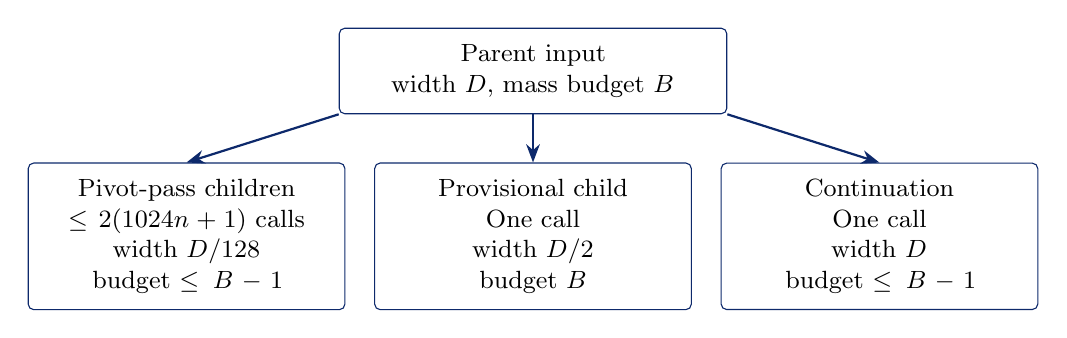
\begin{tikzpicture}[
 >=Stealth,
 box/.style={draw=linkblue,rounded corners=2pt,align=center,
             font=\small,inner sep=6pt,text width=3.6cm},
 edge/.style={->,draw=linkblue,thick}]
 \node[box,text width=4.5cm] (root) at (0,0)
   {Parent input\\width $D$, mass budget $B$};
 \node[box] (loops) at (-4.4,-2.1)
   {Pivot-pass children\\$\le 2(1024n+1)$ calls\\
    width $D/128$\\budget $\le B-1$};
 \node[box] (middle) at (0,-2.1)
   {Provisional child\\One call\\width $D/2$\\budget $B$};
 \node[box] (last) at (4.4,-2.1)
   {Continuation\\One call\\width $D$\\budget $\le B-1$};
 \draw[edge] (root.south west) -- (loops.north);
 \draw[edge] (root.south) -- (middle.north);
 \draw[edge] (root.south east) -- (last.north);
\end{tikzpicture}

 \caption{Children of a nonbase call. The two passes together produce
 at most $2(1024n+1)$ narrow children, each decreasing $B$.
 The provisional child preserves $B$ and halves the width; the
 continuation preserves the box and decreases $B$. Edges show the
 recursion tree, not the execution order.}
 \label{fig:recursion}
\end{figure}

\section{Why the labels satisfy every witness}
\label{sec:correctness}

Termination supplies a well-founded order for the correctness proof.
At a nonbase call, assume that all children satisfy the simultaneous
labelling guarantee. We will show first that the marks $I_-$ and
$I_+$ can safely receive their prescribed labels. We will then show
that every witness with a remaining claim survives the mass change.
These two statements allow the continuation to finish the call.

In the next three lemmas, fix a nonbase input $(A,D,a,b)$ and assume
Theorem~\ref{thm:labelling} for all its children. Witnesses, supports,
and claims without a prime refer to this parent input. Peaks and gaps
are those of Equations~\eqref{eq:max-gaps}--\eqref{eq:min-gaps}.

\subsection{Protection during motion and mass at stopping}

\begin{lemma}[The downward pass]
\label{lem:down}
For every relevant Max witness $x$, its peak $s_x(k)$ is constant
throughout Step~3 and at most $D/2$. In particular, no Max witness
claims an index in $I_-$. For every Min witness $y$ that has a claim
outside $I_-$,
\begin{equation}
             b\bigl(\{i:g_i^y(k^{\downarrow})<q\}\bigr)>3/4.
 \label{eq:down-heavy}
\end{equation}
\end{lemma}

\begin{proof}
Fix $x$ and consider one downward update from pivot $k$. Its
width-$q$ translation is a witness for the child, since that child
keeps Max masses $a$. By Lemma~\ref{lem:translation}, every
coordinate of gap at most $q/32=p$ is a Max claim of the translated
witness. The child's guarantee labels these coordinates $+$, and
they do not move. In particular at least one gap-zero coordinate
continues to attain the old peak.

At every other coordinate, the downward movement $\delta_i$ lies
in $[0,p]$. For its gap $g_i^x(k)>p$,
\[
 x_i-k_i^{\mathrm{new}}
           =s_x(k)-g_i^x(k)+\delta_i<s_x(k).
\]
Thus no coordinate can overtake the old peak, even though many may
move in the same update. The peak is unchanged. Initially $k=c$
and $x\le A+D$, so $s_x(c)\le D/2$. If $x$ claims $i$,
\[
 k_i^{\downarrow}\ge x_i-D/2
                    \ge A_i+D/2-P=c_i-P,
\]
which excludes $i$ from $I_-$.

For the mass assertion, let $y$ claim $j\notin I_-$. The stopped
pivot satisfies $k_j^{\downarrow}\ge c_j-P$, and the claim gives
$y_j\le A_j+P$. Hence
\begin{equation}
 s_y(k^{\downarrow})\ge D/2-2P>D/2-M.
 \label{eq:down-uncapped}
\end{equation}
A coordinate at the lower cap would have
$k_i^{\downarrow}-y_i\le D/2-M$, since $y_i\ge A_i$.
Every maximizer of $k_i^{\downarrow}-y_i$ is therefore strictly
above its cap.

Suppose the mass in Equation~\eqref{eq:down-heavy} were at most
$3/4$. The width-$q$ Min translation has exactly that support, so
it would have support mass at most one for the last child's masses
$\frac43 b$. Its gap-zero maximizers would all have to receive
$-$. At least one of those coordinates would then move down by a
positive amount, because it is above the cap and $p>0$. This
contradicts the final unchanged update. Equality at $3/4$ also
leads to this contradiction, proving the strict mass bound.
\end{proof}

The downward marks are now safe, but the pivot will still move upward.
The next lemma both protects the other type of claim and shows why the
first mass certificate survives that later movement.

\begin{lemma}[The upward pass]
\label{lem:up}
For every relevant Min witness $y$, its peak $s_y(k)$ is constant
throughout Step~4 and at most $D/2$. Thus no Min witness claims an
index in $I_+$. At the final pivot,
\begin{align}
 b\bigl(\{i:g_i^y(k^f)<q\}\bigr)&>3/4
   &&\text{if }y\text{ has a claim outside }I_-;
   \label{eq:final-min-heavy}\\
 a\bigl(\{i:g_i^x(k^f)<q\}\bigr)&>3/4
   &&\text{if }x\text{ has a claim outside }I_+.
   \label{eq:final-max-heavy}
\end{align}
\end{lemma}

\begin{proof}
In every upward child the Min masses are unchanged. Translate a fixed
relevant Min witness $y$ to that width-$q$ box. All gaps at most
$p$ become Min claims, so those coordinates are labelled $-$ and
stay fixed. Every other coordinate has gap greater than $p$ and
moves upward by at most $p$. Its new deviation $k_i^{\mathrm{new}}-y_i$
is therefore strictly below the old peak. A gap-zero coordinate does
not move, proving exact peak preservation. At the start,
$k^{\downarrow}\le c$ and $y\ge A$ imply $s_y\le D/2$.
A Min claim at $i$ consequently gives
\[
                    k_i^f\le y_i+D/2\le c_i+P,
\]
so it is outside $I_+$.

Each coordinate $k_i$ is nondecreasing during this pass while $s_y$
is fixed. It follows that
\begin{equation}
                  g_i^y(k^f)\le g_i^y(k^{\downarrow}).
 \label{eq:min-gap-persistence}
\end{equation}
The set of Min gaps $<q$ can only grow. Its $b$-mass was greater
than $3/4$ at $k^{\downarrow}$ whenever $y$ had a claim outside
$I_-$, by Lemma~\ref{lem:down}. Positivity of $b$ proves
Equation~\eqref{eq:final-min-heavy}.

It remains to obtain the Max mass certificate at this second stopping
point. If $x$ claims $j\notin I_+$, then
$x_j\ge A_j+D-P$ and $k_j^f\le c_j+P$, giving
\[
                      s_x(k^f)\ge D/2-2P>D/2-M.
\]
At an upper-capped coordinate, the inequalities
$k_i^f=c_i+M$ and $x_i\le A_i+D$ would give a deviation at
most $D/2-M$. Thus every maximizer lies strictly below the upper
cap. If the $a$-mass of the gaps $<q$ were at most $3/4$, the
width-$q$ translation would be a Max witness for the final child's
masses $\frac43 a$. Its maximizers would receive $+$ and force a
positive upward movement, contradicting the unchanged update.
This proves Equation~\eqref{eq:final-max-heavy}.
\end{proof}

The mass bounds are absolute: each qualifying set has mass greater
than $3/4$, while the entire witness support has mass at most one.
They are not merely fractional lower bounds relative to a support
that might have much smaller mass. This strength is exactly what
the reweighting calculation needs.

\subsection{Preserving the unsettled witnesses}

The provisional child does not directly label the parent's claims.
Its purpose is to assign the favorable label on each large-mass set
identified above. The larger width $D/2$ makes these sets claims of
the translated witnesses.

\begin{lemma}[Witness survival]
\label{lem:reweight}
Every parent Max witness with a claim outside $I_+$ remains a Max
witness for $(A,D,\bar a,\bar b)$. Every parent Min witness with
a claim outside $I_-$ remains a Min witness for that input.
\end{lemma}

\begin{proof}
Write $r=D/2$ for the provisional width. Since
\[
                         q=D/128<r/32=D/64,
\]
the translated width-$r$ witness claims every coordinate whose parent
gap is $<q$.

For a Max witness $x$ as in the statement, let
$N_x=\{i:g_i^x(k^f)<q\}$ and
$Q_+=\{i:\lambda_i^0=+\}$. Lemma~\ref{lem:up} gives
$a(N_x)>3/4$. By Lemma~\ref{lem:translation}, $N_x\subseteq S_x$;
its coordinates are claims of the width-$r$ translation, which
qualifies for the unchanged masses $a$. Correctness of that child
therefore implies $N_x\subseteq Q_+$. Reweighting the original
support gives
\begin{align*}
 \bar a(S_x)
   &=\frac85 a(S_x)-\frac45 a(S_x\cap Q_+)\\
   &<\frac85\cdot1-\frac45\cdot\frac34=1.
\end{align*}
The continuation has the same box and operator, so the subsolution
inequalities are unchanged. The displayed support bound is all that
is needed to keep $x$ a witness.

For Min set $N_y=\{i:g_i^y(k^f)<q\}$ and
$Q_-=\{i:\lambda_i^0=-\}$. The same two lemmas show
$N_y\subseteq S_y\cap Q_-$ and $b(N_y)>3/4$. Hence
\[
 \bar b(S_y)=\frac85 b(S_y)-\frac45 b(S_y\cap Q_-)
                         <\frac85-\frac45\cdot\frac34=1.
\]
The supersolution inequalities still hold in the unchanged box,
so $y$ also survives.
\end{proof}

\subsection{Completing the simultaneous induction}

\begin{proof}[Proof of Theorem~\ref{thm:labelling}]
Use induction on $R=d+B(\mu)$ from
Lemma~\ref{lem:termination}, which has already established
termination. We prove that a single returned vector meets every
parent obligation.

In the mass base case, $a_i b_i>1$ at every vertex. If $b_i>1$,
no Min witness can contain $i$ in its support, and hence no Min
witness can claim it; returning $+$ is permitted. If $b_i\le1$,
then $a_i>1$, so no Max witness can claim that vertex; returning
$-$ is permitted. This proves all simultaneous obligations in
Step~1.

In the width base case, comparison with the computed box solution
$z$ gives $x\le z\le y$ for every Max witness $x$ and Min
witness $y$. At a Max claim,
\[
                   z_i\ge A_i+D-P>A_i+D/2,
\]
and Step~2 returns $+$. At a Min claim,
$z_i\le A_i+P<A_i+D/2$, and it returns $-$. The argument
also applies to $D=1$, for which the midpoint is a rational
threshold rather than an integer coordinate.

In a nonbase call, all children have smaller rank and satisfy the
simultaneous guarantee by induction. The hypotheses of
Lemmas~\ref{lem:down}--\ref{lem:reweight} therefore hold. Fix
any Max witness and any index $i$ it claims. Lemma~\ref{lem:down}
excludes $i$ from $I_-$. If $i\in I_+$, the positive override
settles it. Otherwise that witness has a claim outside $I_+$ and
survives reweighting by Lemma~\ref{lem:reweight}. The continuation
must label $i$ positively, and no override changes it.

For any Min claim, Lemma~\ref{lem:up} excludes $I_+$. A claim
in $I_-$ receives the negative override. A claim outside $I_-$
belongs to a surviving Min witness and receives $-$ from the
continuation, with no later change. The marks $I_-$ refer to the
earlier pivot, but their safety was proved for the fixed parent
witnesses and remains valid after the upward pass. The two marked
sets may intersect; that intersection contains no claim of either
type, so the stipulated negative precedence causes no conflict.

Every vertex receives exactly one label. Since the witnesses and
claimed indices in the preceding argument were arbitrary, all their
obligations hold together. This completes the induction.
\end{proof}

\section{Counting calls and bit operations}
\label{sec:complexity}

Correctness now gives the complete winning set. To finish the theorem,
we must bound the work in terms of binary input length rather than the
numerical width of the box. There are two relevant depths: the width
can be halved polynomially many times in $L$, but the mass budget can
decrease only logarithmically many times in $n$. Because only one
child preserves that budget, these depths give a quasipolynomial call
count. We then bound the exact arithmetic within each call.

\subsection{The recursion tree}

For the initial data of Equation~\eqref{eq:main-call}, write
\begin{equation}
 d_0=\log_2 D_0,\qquad B_0=B(1/n^2),\qquad
 H=d_0+B_0,\qquad s=2048n+3.
 \label{eq:initial-resources}
\end{equation}
The minimum initial mass product is $1/n^2$. Every path in the call
tree has at most $H$ edges by the rank decrease of
Lemma~\ref{lem:termination}. At most $B_0$ of its edges can
decrease $B$, even if an individual edge decreases it by more than
one. At any node there is at most one child preserving $B$,
namely the provisional child. There are at most $2(1024n+1)$ loop
children and one continuation, so at most $s$ children decrease $B$.

\begin{lemma}[Number of calls]
\label{lem:node-count}
The complete main computation makes at most
\begin{equation}
 \sum_{\ell=0}^{H}\sum_{j=0}^{\min(\ell,B_0)}
       \binom{\ell}{j}s^j
 \ \le\ (H+1)(B_0+1)(1+Hs)^{B_0}
 \label{eq:node-bound}
\end{equation}
calls, including the initial call.
\end{lemma}

\begin{proof}
Consider a node at depth $\ell$ whose path uses $j$ budget-decreasing
edges. Their positions can be chosen in $\binom{\ell}{j}$ ways.
Order each node's budget-decreasing children by execution order.
At each chosen position there are at most $s$ choices of that ordinal; at each
other position there is at most one. This specifies at most
$\binom{\ell}{j}s^j$ possible nodes. Sum over all depths
$0\le\ell\le H$ and $0\le j\le\min(\ell,B_0)$.
For the second inequality, each summand is at most
$(Hs)^j\le(1+Hs)^{B_0}$ and there are at most
$(H+1)(B_0+1)$ summands.
\end{proof}

This count uses the same recursion principle as the reduced-precision
analysis of Parys~\cite[Section~5]{Parys2019}, further developed in
\cite{LehtinenParysScheweWojtczak2022}: one child retains the bounded
parameter while all others improve it. Here the two parameters are
the logarithm of an integer width and the budget derived from rational
mass products.

The explicit encoding bounds both $n$ and $m=|E|$ polynomially in
$L+1$, and each original weight has $O(L+1)$ bits. The perturbation
and Equation~\eqref{eq:initial-width} imply
\[
 \log_2(W+1)=O(L+\log(n+1)),\qquad
 d_0=O(L+\log(n+1)).
\]
Since $\rho=32/25$ is a fixed constant greater than one,
\[
 B_0=1+\lfloor\log_{\rho}(n^2)\rfloor
                          =O(1+\log(n+1)).
\]
Thus $H$ and $s$ are polynomial in $L+1$, and
$B_0=O(\log(L+2))$. Taking logarithms in the call bound gives
\begin{equation}
 \begin{split}
 \log_2\bigl(\text{number of calls}\bigr)
 &\le \log_2(H+1)+\log_2(B_0+1)
                         +B_0\log_2(1+Hs)\\
 &=O((\log_2(L+2))^2).
 \end{split}
 \label{eq:quasipoly-calls}
\end{equation}
This includes $n=1$, for which $B_0=1$.

\subsection{Exact representations}

The nested-box property keeps every endpoint and pivot of the main
computation inside $[0,D_0]^V$. Each such coordinate and each width
therefore uses $O(d_0+1)$ bits. In a basic iteration, an intermediate
edge expression is a coordinate plus a transformed weight. It may be
negative, but its signed binary length is
$O(d_0+\log(W+1)+1)$, polynomial in $L+1$.

Represent a mass by a positive numerator and a positive denominator;
reducing fractions is unnecessary. Starting from $1/n$, a mass is
multiplied along any path only by numbers in
\[
                           \{1,4/3,4/5,8/5\}.
\]
Only budget-decreasing edges change the masses, and a path contains
at most $B_0$ such edges. Thus each numerator and denominator has
$O(B_0+\log(n+1))$ bits. Children receive their own copies of the
input masses. In particular, completing one sibling does not multiply
the parent masses before another sibling starts. Testing $a_i b_i>1$
uses integer cross-multiplication, and testing $b_i>1$ or applying a
constant multiplier also uses numbers of polynomial length. All mass
arithmetic is exact.

The proof quantities $B$ and $\mu$, and the peaks, gaps, supports,
and witness vectors, need not be stored or computed. The algorithm
uses neither a logarithm evaluation for its rank nor an oracle for
the existence of a witness. The procedure evaluates $F$ only inside
$\Basic$, by explicit max/min scans of the edge list.

\subsection{Local cost and uniform implementation}

Each call has polynomial nonrecursive work. The mass and width tests
are finite scans with the arithmetic just bounded. If the width base
case applies, $D<4096$, and the imported iteration bound gives
\[
                            1+nD\le1+4095n
\]
evaluations, including the final stability test. Every evaluation
scans the $m$ explicit edges, adds their transformed weights, takes
the relevant extrema, and clips at $n$ endpoints. It acts on integers
of polynomial length. The midpoint comparison is implemented as
$2z_i>2A_i+D$, which also handles $D=1$.

In a nonbase call, the constants defining the pivot are obtained by
exact divisions by powers of two. Each pass has $O(n+1)$ iterations
apart from its children's work. A scan of the $n$ coordinates performs
one simultaneous update and tests whether it changed anything.
Preparing child inputs and receiving their labels, forming $I_-$
and $I_+$, reweighting, and applying the final overrides likewise
use polynomially many operations on polynomial-length integers.
Schoolbook arithmetic suffices throughout.

A depth-first implementation runs children sequentially and retains
one record per active call. The record holds the parent masses,
endpoints, pivot, labels, and current loop position. There are at most
$H+1$ active records, each of polynomial size. Stack management is
therefore included in the same polynomial local bound. Preprocessing
the transformed weights, finding the least power of two in
Equation~\eqref{eq:initial-width}, and creating masses $1/n$ take
polynomial time. Reading the input and producing the $n$ final labels
also do so.

Multiply this polynomial per-call cost by the call count bounded in
Equation~\eqref{eq:quasipoly-calls}, and include preprocessing and
output. For an absolute constant $C>0$, the complete bound is
\begin{equation}
                            2^{C(\log_2(L+2))^2}.
 \label{eq:final-bit-bound}
\end{equation}
The constants in the procedure are fixed independently of the game,
and every arithmetic and control operation has been specified. This
gives a uniform deterministic bit algorithm.

\begin{proof}[Proof of Theorem~\ref{thm:main}]
Compute Equation~\eqref{eq:main-call}, run $\Label$, and output
the positively labelled vertices. Theorem~\ref{thm:labelling}
guarantees the labels required by every witness. In the initial box,
the box solution is a witness of both types, and the argument after
Equation~\eqref{eq:main-call} identifies all its required labels
with the bands of Proposition~\ref{prop:game-reduction}. The
positive band is exactly the zero-threshold winning set, including
against every history-dependent opponent. Equation~\eqref{eq:final-bit-bound}
bounds the entire computation. Signed binary weights, self-loops,
and separately listed parallel edges are all covered by the
construction and accounting above.
\end{proof}

\section{Exact values and optimal positional strategies}
\label{sec:full-solution}

We now use the winning-set algorithm to recover the numerical values
and strategies of the game. For the input model of
Theorem~\ref{thm:main}, write
\[
 \operatorname{val}_w(v)
 =\sup_\sigma\inf_\tau \MP_w(\pi_{v,\sigma,\tau}),
\]
where the strategies may depend on the full finite history.

\begin{corollary}[Full game solution]\label{cor:full-solution}
A uniform deterministic algorithm returns the exact value
$\operatorname{val}_w(v)$ as a reduced rational for every $v\in V$
and one positional strategy $\sigma^\star$ for Max and one positional
strategy $\tau^\star$ for Min such that, simultaneously for every
$v\in V$ and every pair of history-dependent strategies $\sigma,\tau$,
\[
 \MP_w(\pi_{v,\sigma^\star,\tau})\ge\operatorname{val}_w(v),
 \qquad
 \MP_w(\pi_{v,\sigma,\tau^\star})\le\operatorname{val}_w(v).
\]
The complete computation takes
$2^{O((\log_2(L+2))^2)}$ bit operations.
\end{corollary}

\begin{proof}
\noindent\textbf{Positional values.}\enspace
The uniform form of Ehrenfeucht--Mycielski positional determinacy
\cite{EhrenfeuchtMycielski1979}, stated explicitly in
\cite[Theorem~1 and the following paragraph]{BrimEtAl2011}, provides
one positional strategy for each player attaining the value from all
vertices at once, against arbitrary history-dependent opponents.
The latter source uses an edge relation without parallel entries.
For our convention, replace each explicit edge $e:u\to v$ by
$u\to x_e\to v$ through a fresh vertex with a single outgoing edge,
with weights $2w(e)$ and $0$. Keep ownership at the original vertices;
the owner of $x_e$ is immaterial. The resulting graph has no parallel
edges or loops. Expanded histories retain the identity of every
original edge. Their averages at even prefixes equal the original
averages, and the odd-prefix discrepancy tends to zero. Thus payoffs
and the uniform positional guarantees transfer back to our graph,
including loops and parallel entries.

Set $W_{\mathrm{in}}=\max_{e\in E}|w(e)|$. Fix both uniform optimal
positional strategies. From any vertex the resulting play eventually
repeats a simple directed cycle of at most $n$ edges in the original
graph, and its mean is the value at that vertex. Consequently every
value has a reduced representation $a/b$ with
\[
 1\le b\le n,\qquad |a|\le bW_{\mathrm{in}},
 \qquad -W_{\mathrm{in}}\le a/b\le W_{\mathrm{in}}.
\]
The same bounds hold after restricting outgoing choices, provided at
least one outgoing edge remains at every vertex.

\par\medskip\noindent\textbf{Threshold queries and exact reconstruction.}\enspace
We use the classical reduction from values to threshold queries
\cite[Section~5.2]{BrimEtAl2011}, keeping track of binary lengths.
For integers $p$ and $q>0$, replace each weight by
$w_{p/q}(e)=qw(e)-p$. For every infinite play,
\[
 \MP_{w_{p/q}}(\pi)=q\MP_w(\pi)-p.
\]
Positional attainment therefore makes the winning set returned by
Theorem~\ref{thm:main} exactly
$\{v:\operatorname{val}_w(v)\ge p/q\}$.

Choose
$K=1+\lceil\log_2(2(W_{\mathrm{in}}+1)n^2)\rceil$, computable from
integer bit lengths. For each vertex, start with the closed interval
$[-W_{\mathrm{in}},W_{\mathrm{in}}]$ and make $K$ bisections. Query
its midpoint and move the lower endpoint to the midpoint if the
vertex belongs to the returned set; otherwise move the upper endpoint.
The final interval contains its value and has width
$2W_{\mathrm{in}}2^{-K}<1/n^2$. Distinct reduced rationals with
positive denominators at most $n$ differ by at least $1/n^2$.
To reconstruct the value from an interval $[\ell,h]$, for each
$1\le b\le n$ test the integer $a=\lceil b\ell\rceil$ for
$a/b\le h$, reduce the retained fractions, and remove repetitions.
Since $b(h-\ell)<1$, this tests every possible numerator.
The value bound above guarantees exactly one resulting rational.
Call this value-vector procedure $\mathsf{Values}(H)$ for any
restricted game $H$; the original $n,W_{\mathrm{in}},K$ remain valid
for all such calls.

\par\medskip\noindent\textbf{Separate strategy self-reductions.}\enspace
An edge joining vertices of the same value need not be optimal.
For example, let a Max vertex $u$ have a zero-weight self-loop and a
zero-weight edge to a vertex $v$ whose only edge is a self-loop of
weight $1$. Both vertices have value $1$, but staying at $u$ yields
payoff $0$. We therefore test restrictions of the current game and
preserve its entire value vector.

First compute $\mathbf v=\mathsf{Values}(G)$. For Max, start from a
fresh copy $H=G$ and process the Max vertices in any fixed order.
At a vertex $u$, form a trial $H_e$ for each outgoing edge $e$ by
keeping only $e$ at $u$. Keep a trial for which
$\mathsf{Values}(H_e)=\mathbf v$, and continue from that trial.
Such an edge always exists. Indeed, take the edge chosen at $u$ by a
globally optimal positional Max strategy of the current $H$.
Restricting Max's choices cannot increase any value, while that
strategy remains available and secures the current entire value
vector, so no value decreases either. This proves the invariant
$\mathsf{Values}(H)=\mathbf v$.

At the end, Max has one allowed edge at every owned vertex, whereas
all of Min's original choices remain. The resulting single Max
strategy therefore secures $\mathbf v$ from every vertex against
every Min strategy. To recover Min's strategy, start again from a
fresh copy of the original $G$, not from the Max-restricted game.
At each Min vertex keep an outgoing edge whose trial preserves
$\mathbf v$. A globally optimal positional Min strategy of the
current game supplies such an edge: restricting Min cannot decrease
values, and that strategy prevents any increase. The final Min
strategy is optimal against every original Max strategy. Thus the two
separately recovered strategies have the simultaneous guarantees in
the statement.

\par\medskip\noindent\textbf{Call and bit bounds.}\enspace
Put $m=|E|$. At a vertex, at most its original outdegree many trials
are tested, so the two self-reductions together use at most $m$ trial
value-vector computations. Including the original computation, there
are at most
\begin{equation}
 Q=nK(1+m)
 \label{eq:threshold-call-bound}
\end{equation}
threshold calls. Every midpoint has denominator dividing $2^K$ and
a numerator of $O(\log(W_{\mathrm{in}}+1)+K)$ bits. Each transformed
weight has the same order of bit length. Since
$K=O(L+\log(n+1))$, the full encoding length of every queried game
is $O(L+mK)$, polynomial in $L+1$. Reconstruction, reduced-rational
comparison, and copying restricted edge lists also have polynomial
bit cost. The explicit encoding bounds $n,m$ polynomially in $L+1$,
so $Q$ is polynomial. Applying Theorem~\ref{thm:main} to these
polynomial-length games and multiplying by $Q$ gives
$2^{O((\log_2(L+2))^2)}$ bit operations, including the polynomial-size
value and strategy output.
\end{proof}

The preceding reduction also applies to the companion algorithm.
Here the additional issue is that threshold queries depend on earlier
answers, so the winning-set error must be controlled at each query.

\begin{corollary}[Randomized full game solution]
\label{cor:randomized-full-solution}
For the game model of Theorem~\ref{thm:main}, a uniform randomized
algorithm returns all exact values and both globally optimal positional
strategies specified in Corollary~\ref{cor:full-solution} with
probability at least $7/8$ for the entire output. Its running time is
$2^{O((\log_2(L+2))^2)}$ bit operations on every random tape.
\end{corollary}

\begin{proof}
The companion's Theorem~1.1 \cite{OpenAI2026Randomized} returns the
whole winning set correctly with probability at least $7/8$ and has
the quasipolynomial bit bound on every tape. Use the reduction above,
whose number of threshold queries is bounded by the polynomial $Q$
in Equation~\eqref{eq:threshold-call-bound}. For each query, take
$r=2\lceil\log_2(8Q)\rceil+1$ independent fresh runs and use the
coordinatewise majority of their winning sets. Conditional on the
previous history, the current query is fixed. The amplified set is
correct whenever more than half of the runs return the whole correct
set, and its conditional failure probability is at most
\[
 \sum_{j=\lceil r/2\rceil}^{r}\binom rj(1/8)^j
 \le 2^r(1/8)^{r/2}=2^{-r/2}<\frac1{8Q}.
\]
A first-error union bound over the adaptive queries makes every
threshold answer correct with probability at least $7/8$. On this
event the preceding deterministic argument gives all exact values and
both globally optimal strategies. On other tapes, if reconstruction
does not yield a unique rational or no value-preserving trial is
found, the reduction stops with zero at every value coordinate and
the first listed outgoing edge at every owned vertex.
All loops have the stated caps even then. Since $r=O(\log(L+2))$ and
all queried encodings retain their polynomial bound on every tape,
the total bit bound remains quasipolynomial on every tape, including
random-bit generation. This transfer uses only the winning-set
interface.
\end{proof}

\section{Fixed- and minimum-credit energy games}
\label{sec:energy-credits}

The preceding algorithms also compute the initial credits needed in
one-resource energy games. Retain the game model of
Theorem~\ref{thm:main}. For a start $v\in V$ and an integer credit
$c\ge0$, call
$(v,c)$ \emph{energy-winning} if Max has a strategy such that, against
every history-dependent Min strategy, the induced play satisfies
\begin{equation}
 c+\sum_{t=0}^{j-1}w(e_t)\ge0\qquad\text{for every }j\ge0.
 \label{eq:energy-objective}
\end{equation}
There is one accumulated resource and no upper bound or saturation.
Write $c_{\min}(v)$ for the least nonnegative integer credit for which
$(v,c)$ is energy-winning, and put $c_{\min}(v)=\infty$ if there is
none. A positional Max policy specifies one labelled outgoing edge at
each Max vertex.

The reductions connecting these problems to mean-payoff games are
classical. Bouyer, Fahrenberg, Larsen, Markey, and Srba formulate the
fixed-credit lower-bound problem and reduce it to mean payoff using
adversary-controlled returns to the start
\cite[Section~2.1 and Proposition~12]{BouyerEtAl2008}. Our construction
places the initial credit on each return edge. Brim, Chaloupka, Doyen,
Gentilini, and Raskin distinguish the unknown-credit and minimum-credit
problems, record the unknown-credit/mean-payoff equivalence, and
characterize minimum credits by an energy progress measure
\cite[Section~2 and Theorems~3 and~5]{BrimEtAl2011}. The reset construction
below lets us apply Corollary~\ref{cor:full-solution} to a prescribed-credit
instance, recovering a policy when that instance is winning. A bound on
finite minimum credits then permits exact binary search.

\begin{corollary}[Fixed and minimum energy credits]
\label{cor:energy-credits}
Uniform deterministic algorithms have the following guarantees.
\begin{enumerate}
\item Given $v$ and a nonnegative binary integer $c$, decide whether
$(v,c)$ is energy-winning. On a positive answer, return a positional
Max policy satisfying Equation~\eqref{eq:energy-objective} from that
start and credit against every history-dependent Min strategy.
\item Given $v$, return the exact $c_{\min}(v)$, including the possible
answer $\infty$. On a finite answer, return a positional Max policy
winning from $v$ at credit $c_{\min}(v)$.
\end{enumerate}
The fixed-credit computation takes
$2^{O((\log_2(L_c+2))^2)}$ bit operations, where $L_c$ is the full
explicit input length including the start and credit. The
minimum-credit computation takes $2^{O((\log_2(L+2))^2)}$ bit
operations for the original game length $L$. Handling every vertex by
separate per-start searches, including a separate policy
for every finite answer, has the same form of total bit bound.

Each policy may depend on the queried start and credit; it also wins
from that same start at every larger credit.
\end{corollary}

\begin{proof}
\noindent\textbf{Fixed credit by resetting.}\enspace
For the fixed pair $(v,c)$ construct a mean-payoff game $R_{v,c}$.
Replace every $u\in V$ by an entry $u_{\mathrm{in}}$ owned by Min and
an exit $u_{\mathrm{out}}$ owned by the original owner of $u$. Add the
two edges
\[
 u_{\mathrm{in}}\xrightarrow{c}v_{\mathrm{in}},
 \qquad
 u_{\mathrm{in}}\xrightarrow{0}u_{\mathrm{out}},
\]
and replace each labelled original edge $e:u\to z$ by its own edge
\[
 u_{\mathrm{out}}\xrightarrow{w(e)}z_{\mathrm{in}}.
\]
Start at $v_{\mathrm{in}}$. The game is total and has $2n$ vertices
and $m+2n$ edges, where $m=|E|$. The reset at $u=v$ is a nonnegative
self-loop, including when $c=0$, and distinct original parallel edges
remain distinct. If $U(R_{v,c})$ denotes its zero-threshold winning
set, then
\begin{equation}
 (v,c)\text{ is energy-winning in }G
 \quad\Longleftrightarrow\quad v_{\mathrm{in}}\in U(R_{v,c}).
 \label{eq:energy-reset-equivalence}
\end{equation}

For the forward implication, use an energy-winning strategy from
$(v,c)$ and restart its history after each reset. In any transformed
prefix, every completed segment has original-edge sum at least $-c$
and then receives the reset weight $+c$. Its total is therefore
nonnegative. The unfinished segment has sum at least $-c$; the
intervening zero edges do not change this bound. Every transformed
prefix sum is consequently at least $-c$. Dividing by its length
shows that the lower limiting average is nonnegative. This argument
also covers no resets and infinitely many resets, and does not assume
that the original energy strategy is positional.

Conversely, if $v_{\mathrm{in}}\in U(R_{v,c})$,
Corollary~\ref{cor:full-solution} returns a positional Max strategy
for $R_{v,c}$ guaranteeing nonnegative mean payoff from that start.
Restrict its choices at Max exits to obtain a positional policy in
$G$. Suppose a consistent original prefix of length $j$ from $v$ had
weight $q<-c$. In the reset game Min can choose continuation at its
entries, follow that prefix at its owned exits, and then reset. This
is a closed walk from $v_{\mathrm{in}}$ with weight $q+c<0$ and
length $2j+1$. Positionality of the Max strategy makes the same walk
consistent on every repetition. Min could therefore repeat it forever,
giving mean payoff $(q+c)/(2j+1)<0$, a contradiction. Thus all original
prefixes have weight at least $-c$. This proves the equivalence and
the positive-answer policy guarantee; only the Max strategy from the
full-solution call is used.

\par\medskip\noindent\textbf{A finite credit bound and exact search.}\enspace
For the original weights put
\begin{equation}
 W_{\mathrm{in}}=\max_{e\in E}|w(e)|,
 \qquad H=(n-1)W_{\mathrm{in}}.
 \label{eq:energy-credit-bound}
\end{equation}
In particular $W_{\mathrm{in}}$ and $H$ may be zero. An energy winner
with any finite credit is an original zero-threshold mean-payoff
winner, since its prefix sums are bounded below. Conversely, the
cycle-deletion estimate in the proof of
Proposition~\ref{prop:game-reduction} gives a positional Max policy
on the original winning region for which every consistent prefix has
weight at least $-H$. Indeed, its permitted simple cycles have
nonnegative original sum, and deleting such cycles from a prefix leaves
at most $n-1$ edges, each of weight at least $-W_{\mathrm{in}}$.
Consequently, for the original winning set $U(G)$,
\begin{equation}
 c_{\min}(v)<\infty\quad\Longleftrightarrow\quad v\in U(G),
 \qquad
 v\in U(G)\quad\Longrightarrow\quad 0\le c_{\min}(v)\le H.
 \label{eq:energy-finite-equivalence}
\end{equation}
The algorithm uses this existence bound as a known winning endpoint;
it need not compute the potential used in that proposition.

Compute $U(G)$ once by Theorem~\ref{thm:main} and output $\infty$ for
starts outside it. For a winning start, the fixed-credit predicate is
monotone: a strategy that wins at $c$ still wins at every larger
credit. Binary search with a formal losing lower endpoint $\ell=-1$
and the known winning upper endpoint $h=H$. While $h-\ell>1$, query
$\lfloor(\ell+h)/2\rfloor$ by
Equation~\eqref{eq:energy-reset-equivalence} and replace the endpoint
having the same answer. The sentinel itself is never queried. This takes at most
$\lceil\log_2(H+1)\rceil$ fixed-credit decisions and returns the exact
least winning integer. When $H=0$ the initial gap is one, so no search
query is made and the answer is zero. This includes both $n=1$ and
all-zero weights; any start without a finite credit has already been
excluded by $U(G)$. To return a policy at the minimum, apply
Corollary~\ref{cor:full-solution} to $R_{v,c_{\min}(v)}$ and restrict
its Max choices as above.

\par\medskip\noindent\textbf{Bit complexity and output size.}\enspace
Let $b_c$ be the binary length of the supplied nonnegative credit,
so $b_c=O(1+\log_2(c+1))$. The explicit reset game has encoding length
\[
 O\bigl(L+n(b_c+\log_2(n+1))\bigr),
\]
which is polynomial in $L_c$. The credit is copied into only $n$ edge
records; no array indexed by its numerical value is constructed.
Theorem~\ref{thm:main} decides membership in its winning set, and a
single application of Corollary~\ref{cor:full-solution} on a positive
answer supplies the policy, within the fixed-credit bound claimed.

For minimum credits, $H$ and every queried credit have
$O(1+\log_2(n+1)+\log_2(W_{\mathrm{in}}+1))=O(L+1)$ bits. All queried
encodings therefore have polynomial length in $L+1$. For all vertices,
the outer reduction makes at most $1+n\lceil\log_2(H+1)\rceil$ direct
winning-set calls, including the original one, and at most one
full-solution call for each requested finite-credit policy. These
counts are polynomial in
$L+1$. Polynomially many calls on polynomial-length inputs preserve
$2^{O((\log_2(L+2))^2)}$ bit complexity. Computing $H$, the binary
search arithmetic, and copying the policies have polynomial bit cost.
The output also has polynomial length: each finite credit has the
stated bit bound, and each per-start policy lists one original edge
at each Max vertex. No energy-indexed array is used in the search.
\end{proof}

\section{Tropical feasibility and fixed corank}
\label{sec:tropical}

Akian, Gaubert, and Guterman identify the coordinates that can be finite
in a solution of tropical inequalities with the winning states of an
associated mean-payoff game
\cite[Theorem~3.2 and Corollary~3.7]{AkianGaubertGuterman2012}.
Together with Theorem~\ref{thm:main}, this gives binary-length bounds
for tropical feasibility and for rank within a fixed distance of the
number of columns. We use the conventions $a+(-\infty)=-\infty$
and $\max\varnothing=-\infty$.

\begin{corollary}[Tropical feasibility and fixed corank]
\label{cor:tropical-computation}
For explicitly listed $m\times n$ matrices $A,B$ and $m$-dimensional
vectors $c,d$ over $\mathbb Q\cup\{-\infty\}$, feasibility of
\[
 \max\bigl\{c_i,\max_j(A_{ij}+x_j)\bigr\}
 \leq \max\bigl\{d_i,\max_j(B_{ij}+x_j)\bigr\}
 \qquad\text{for every row }i
\]
is decidable deterministically in
$2^{O((\log(L+2))^2)}$ bit operations, where $L$ is the complete
explicit binary input length. Variables range over
$\mathbb R\cup\{-\infty\}$; feasibility with all coordinates finite
is decidable within the same bound. Equalities between the two displayed
maxima are allowed, interpreted as pairs of inequalities.
For a homogeneous system ($c=d=-\infty$), one can also compute the
maximal finite-coordinate support of a solution, including the empty
support. In particular, the same bound decides feasibility of max-atom
systems $z\leq\max(x,y)+a$, with rational constants $a$ and finite
real, equivalently rational, variables.

For each fixed integer $k\geq0$, a deterministic algorithm with bit
bound $2^{O_k((\log(L+2))^2)}$ decides whether an explicitly listed
$m\times n$ matrix over $\mathbb Q\cup\{-\infty\}$, with $m\geq n\geq1$,
has tropical rank at least $n-k$. Here tropical rank is the largest
order of a square submatrix whose permutation sums have a finite,
unique maximum.
The rank is zero if no such nonempty submatrix exists.
\end{corollary}

\begin{proof}
\noindent\textbf{Integer data and homogeneous supports.}\enspace
Let $Q$ be the product of the positive denominators of the finite input
coefficients, taking $Q=1$ when there are none. Multiplying every finite
coefficient and variable by $Q$ preserves the inequalities and the sets
of finite coordinates. It also preserves the comparisons between
permutation sums that define tropical rank. The bit length of $Q$ is
at most one plus the sum of the denominator bit lengths, so the scaled integer
data have polynomial binary length.

Consider first a homogeneous system
\begin{equation}
 \max_j(C_{ij}+z_j)\leq\max_j(D_{ij}+z_j)
 \qquad\text{for every }i.
 \label{eq:tropical-homogeneous}
\end{equation}
The support of $z$ is $\{j:z_j\ne-\infty\}$. To obtain a total game,
apply the preprocessing of \cite[Section~2.1]{AkianGaubertGuterman2012}.
Discard a row whose left side is identically $-\infty$. If a right
side is identically $-\infty$, every variable with a finite coefficient
on that row's left side must equal $-\infty$. Record these coordinates,
substitute $-\infty$ for them throughout the system, and repeat.
Each step removes a row or a variable, so this takes polynomial time.
If no variables remain, the maximal support is empty. Otherwise add
the tautologies $z_j\leq z_j$ for the remaining variables.

The resulting bipartite game has a Min vertex for each remaining column
and a Max vertex for each row. A finite $C_{ij}$ gives an edge from
column $j$ to row $i$ of weight $-C_{ij}$; a finite $D_{ij}$ gives
an edge from row $i$ to column $j$ of weight $D_{ij}$. Every vertex
has an outgoing edge. Theorem~3.2 of
\cite{AkianGaubertGuterman2012} identifies its winning column vertices
with the maximal support of a solution. The recorded deleted coordinates
belong to no support. The union of all supports is attained, because
coordinatewise maxima of finitely many solutions are again solutions;
the identically $-\infty$ solution realizes the empty case.

The cited game counts a column--row--column pair as one turn. Counting
the two edges separately halves the mean payoff; the contribution of
an unmatched edge tends to zero. The source uses upper limiting averages;
positional optimality makes their nonnegative winning set coincide with
that for our lower limiting averages. The game has
polynomially many vertices and edges, with weights copied or negated
from the scaled coefficients or equal to zero. Its full binary encoding
is polynomial in $L+1$, so Theorem~\ref{thm:main} computes the maximal
support within the asserted bound.

\par\medskip\noindent\textbf{Affine and finite feasibility.}\enspace
After scaling, append $c$ to $A$ and $d$ to $B$ as a new column,
and introduce one coordinate $t$. The homogeneous system is
\[
 \max\bigl\{c_i+t,\max_j(A_{ij}+z_j)\bigr\}
 \leq\max\bigl\{d_i+t,\max_j(B_{ij}+z_j)\bigr\}.
\]
Every affine solution $x$ gives a homogeneous solution $(x,0)$.
Conversely, a homogeneous solution with finite $t$ gives the affine
solution $x_j=z_j-t$. Thus affine feasibility asks whether the new
coordinate belongs to the maximal support. Feasibility with all original
coordinates finite asks whether that support contains all $n+1$
coordinates. A coordinate eliminated during preprocessing is absent
from the computed support, so any test requiring it fails; this includes
$t$ if it is forced to $-\infty$.
This is the homogenization underlying
\cite[Theorem~3.5 and Corollaries~3.4 and~3.7]{AkianGaubertGuterman2012}.
Equalities are handled by imposing both inequalities.

A max-atom $z\leq\max(x,y)+a$ is a homogeneous row with one term on
the left and two on the right. Apply the all-finite test. With integer
coefficients, taking the floor of each finite coordinate preserves every
inequality: flooring commutes with integer translation and with finite
maxima. Scaling back therefore gives a rational solution whenever a real
one exists. This also explains the integral-solution interface in
\cite[Proposition~3.9, Corollary~3.10 and Remark~3.15]
{AkianGaubertGuterman2012}.

\par\medskip\noindent\textbf{Fixed corank.}\enspace
If $n\leq k$, the rank threshold is nonpositive and the answer is yes.
Otherwise set $r=n-k$. The rank criterion of
\cite[Corollaries~4.16--4.17]{AkianGaubertGuterman2012} says that the
rank is at least $r$ exactly when some set of $r$ columns is tropically
independent. For each such set let $M$ be the resulting $m\times r$
matrix. Its columns are dependent precisely when there is a vector
$z\not\equiv-\infty$ such that every row maximum is attained at least
twice or equals $-\infty$. Equivalently, $z$ satisfies the homogeneous
system
\begin{equation}
 M_{ij}+z_j\leq\max_{\ell\ne j}(M_{i\ell}+z_\ell)
 \qquad(1\leq i\leq m,\ 1\leq j\leq r).
 \label{eq:tropical-dependence}
\end{equation}
Its maximal support is therefore empty exactly when the selected columns
are independent. This is the inequality form of the game reduction in
\cite[Theorem~4.9]{AkianGaubertGuterman2012}. The row index $(i,j)$
retains the column excluded from Max's next choice. Empty right sides
and all-$-\infty$ columns are covered by the support computation above,
including when $r=1$.

There are at most $mr$ inequalities, with $r$ coefficients on each
side, so each test has polynomial encoding length. There are
$\binom nr=\binom nk\leq n^k$ tests. For fixed $k$, their total
bit cost is $2^{O_k((\log(L+2))^2)}$, as claimed.
\end{proof}

Strongly polynomial algorithms have been claimed using max-atoms and
tropical optimization
\cite{Truffet2025MaxAtoms,Truffet2026SubstitutionV4}.
Appendix~A of the randomized companion gives a two-variable
counterexample to the printed variable-selection rule in
\texttt{arXiv:2603.26423v4}~\cite{OpenAI2026Randomized}.
That comparison is specific to the version and rule examined; it
neither assesses the distinct 2025 max-atom proof nor transfers to
a revised procedure. It has no role in the proofs of this article.

\bibliographystyle{plain}
\bibliography{references}
\end{document}
